\section{Multicore Architectures}

\subsection{Explore the CPU}

\begin{lstlisting}[caption=Output from lscpu command]
-bash-4.1$ lscpu
Architecture:          x86_64
CPU op-mode(s):        32-bit, 64-bit
Byte Order:            Little Endian
CPU(s):                32
On-line CPU(s) list:   0-31
Thread(s) per core:    2
Core(s) per socket:    8
Socket(s):             2
NUMA node(s):          4
Vendor ID:             AuthenticAMD
CPU family:            21
Model:                 1
Model name:            AMD Opteron(TM) Processor 6274
Stepping:              2
CPU MHz:               1400.000
BogoMIPS:              4399.38
Virtualization:        AMD-V
L1d cache:             16K
L1i cache:             64K
L2 cache:              2048K
L3 cache:              6144K
NUMA node0 CPU(s):     0-7
NUMA node1 CPU(s):     8-15
NUMA node2 CPU(s):     16-23
NUMA node3 CPU(s):     24-31
\end{lstlisting}

Based on the output above it seems that the CPU has dualthreaded cores and 8 
cores per cpu. With our two physical cpus this would make 16 cores and 32 virtual
CPUs. But this is an AMD processor and the architecture is a bit different than
it first seems. According to \href{https://www.cpu-world.com/CPUs/Bulldozer/AMD-Opteron%206274%20OS6274WKTGGGU.html}{cpu-world.com}
the CPU actually has 16 physical cores. It has L1 data caches for each core, and 
shared instruction caches for every two cores. The L2 cache is shared between 
two cores as well. L3 Cache is shared among 8 cores. See figure \ref{fig:amd}
for a visual illustration of a single AMD Opetron 6274.

\begin{figure}
    \centering
    \label{fig:amd}
    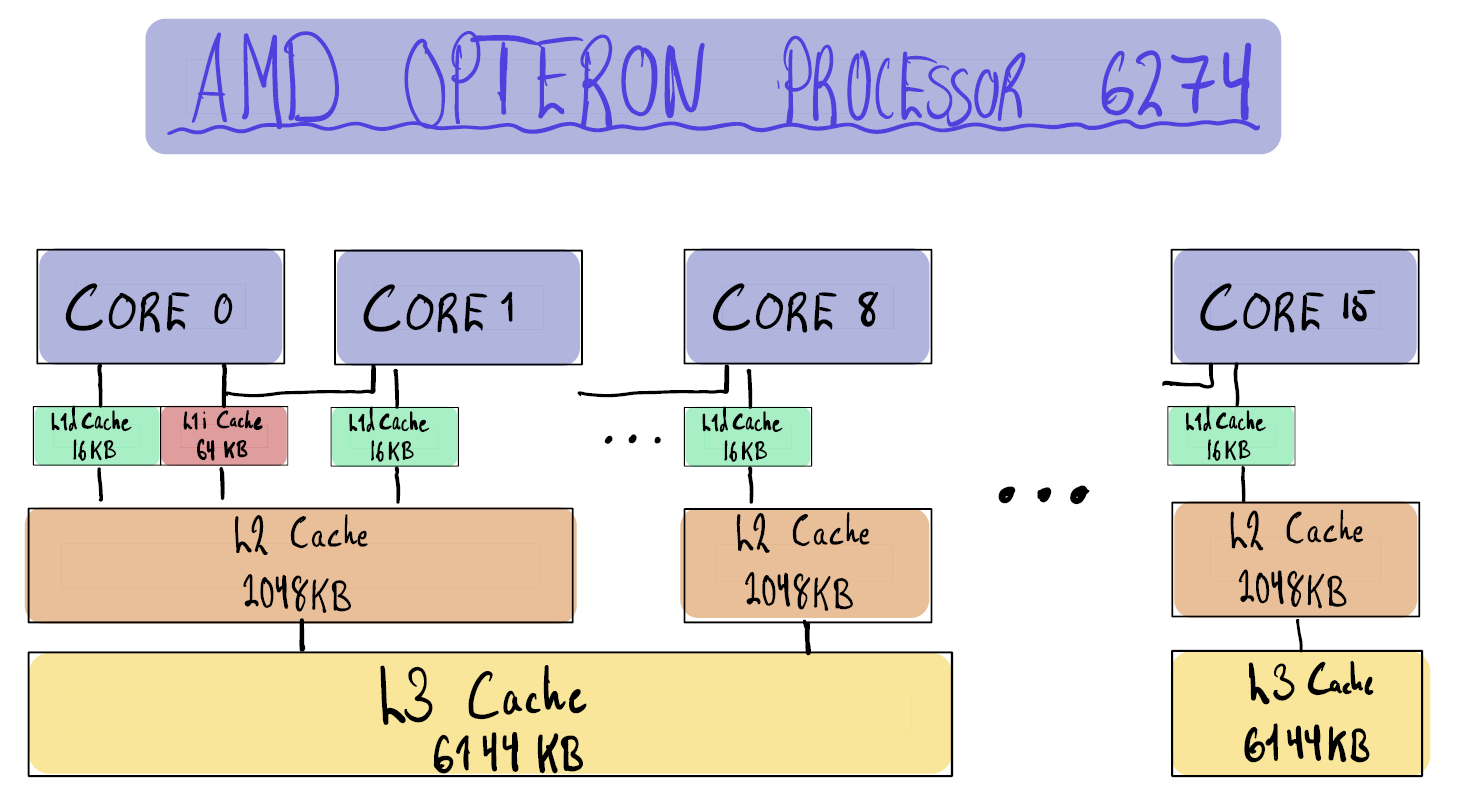
\includegraphics[width=\linewidth]{Figures/datahierarchy.PNG}
    \caption{Cache Hierarchy of AMD Opteron Processor 6274 on gullviva.it.uu.se}
\end{figure}

We see that this processor has a lot more physical cores. In summary we have:

\begin{itemize}
    \item There are in total 2 physical CPUs. Each with 16 physical cores.
    \item Each physical core has an L1d of 16KB
    \item There is an L1i Cache of 64KB for every two cores. 
    \item There is a L2 Cache of 2048KB for every two cores.
    \item Eight physical cores share one L3 cache of size 6144KB.
\end{itemize}

Compared with the Intel cpu the cache levels are the same. The memory split
is what is the main different between the two cpus. There are more physical
cores in the AMD cpu but the instruction memory is shared between the cores. 
The CPU we are using also has a lot more cores than the Intel CPU.